\def\year{2021}\relax
%File: formatting-instructions-latex-2021.tex
%release 2021.2
\documentclass[letterpaper]{article} % DO NOT CHANGE THIS
\usepackage{aaai21}  % DO NOT CHANGE THIS
\usepackage{times}  % DO NOT CHANGE THIS
\usepackage{helvet} % DO NOT CHANGE THIS
\usepackage{courier}  % DO NOT CHANGE THIS
\usepackage[hyphens]{url}  % DO NOT CHANGE THIS
\usepackage{graphicx} % DO NOT CHANGE THIS
\urlstyle{rm} % DO NOT CHANGE THIS
\def\UrlFont{\rm}  % DO NOT CHANGE THIS
\usepackage{natbib}  % DO NOT CHANGE THIS AND DO NOT ADD ANY OPTIONS TO IT
\usepackage{caption} % DO NOT CHANGE THIS AND DO NOT ADD ANY OPTIONS TO IT
\frenchspacing  % DO NOT CHANGE THIS
\setlength{\pdfpagewidth}{8.5in}  % DO NOT CHANGE THIS
\setlength{\pdfpageheight}{11in}  % DO NOT CHANGE THIS

\usepackage[ruled,vlined]{algorithm2e}
 \usepackage{subcaption} % subfigures
\SetKwInOut{Parameter}{parameter}

%\nocopyright
%PDF Info Is REQUIRED.
% For /Author, add all authors within the parentheses, separated by commas. No accents or commands.
% For /Title, add Title in Mixed Case. No accents or commands. Retain the parentheses.
\pdfinfo{
/Title (Latent-CF: A Simple Baseline for Reverse Counterfactual Explanations)
/Author (Rachana Balasubramanian, Sam Sharpe, Bayan Bruss, Brian Barr)
/TemplateVersion (2021.2)
} %Leave this
% /Title ()
% Put your actual complete title (no codes, scripts, shortcuts, or LaTeX commands) within the parentheses in mixed case
% Leave the space between \Title and the beginning parenthesis alone
% /Author ()
% Put your actual complete list of authors (no codes, scripts, shortcuts, or LaTeX commands) within the parentheses in mixed case.
% Each author should be only by a comma. If the name contains accents, remove them. If there are any LaTeX commands,
% remove them.

% DISALLOWED PACKAGES
% \usepackage{authblk} -- This package is specifically forbidden
% \usepackage{balance} -- This package is specifically forbidden
% \usepackage{color (if used in text)
% \usepackage{CJK} -- This package is specifically forbidden
% \usepackage{float} -- This package is specifically forbidden
% \usepackage{flushend} -- This package is specifically forbidden
% \usepackage{fontenc} -- This package is specifically forbidden
% \usepackage{fullpage} -- This package is specifically forbidden
% \usepackage{geometry} -- This package is specifically forbidden
% \usepackage{grffile} -- This package is specifically forbidden
% \usepackage{hyperref} -- This package is specifically forbidden
% \usepackage{navigator} -- This package is specifically forbidden
% (or any other package that embeds links such as navigator or hyperref)
% \indentfirst} -- This package is specifically forbidden
% \layout} -- This package is specifically forbidden
% \multicol} -- This package is specifically forbidden
% \nameref} -- This package is specifically forbidden
% \usepackage{savetrees} -- This package is specifically forbidden
% \usepackage{setspace} -- This package is specifically forbidden
% \usepackage{stfloats} -- This package is specifically forbidden
% \usepackage{tabu} -- This package is specifically forbidden
% \usepackage{titlesec} -- This package is specifically forbidden
% \usepackage{tocbibind} -- This package is specifically forbidden
% \usepackage{ulem} -- This package is specifically forbidden
% \usepackage{wrapfig} -- This package is specifically forbidden
% DISALLOWED COMMANDS
% \nocopyright -- Your paper will not be published if you use this command
% \addtolength -- This command may not be used
% \balance -- This command may not be used
% \baselinestretch -- Your paper will not be published if you use this command
% \clearpage -- No page breaks of any kind may be used for the final version of your paper
% \columnsep -- This command may not be used
% \newpage -- No page breaks of any kind may be used for the final version of your paper
% \pagebreak -- No page breaks of any kind may be used for the final version of your paperr
% \pagestyle -- This command may not be used
% \tiny -- This is not an acceptable font size.
% \vspace{- -- No negative value may be used in proximity of a caption, figure, table, section, subsection, subsubsection, or reference
% \vskip{- -- No negative value may be used to alter spacing above or below a caption, figure, table, section, subsection, subsubsection, or reference

\setcounter{secnumdepth}{0} %May be changed to 1 or 2 if section numbers are desired.

% The file aaai21.sty is the style file for AAAI Press
% proceedings, working notes, and technical reports.
%

% Title

% Your title must be in mixed case, not sentence case.
% That means all verbs (including short verbs like be, is, using,and go),
% nouns, adverbs, adjectives should be capitalized, including both words in hyphenated terms, while
% articles, conjunctions, and prepositions are lower case unless they
% directly follow a colon or long dash

\title{Latent-CF: A Simple Baseline for Reverse Counterfactual Explanations}
\author{
    %Authors
    % All authors must be in the same font size and format.
    Rachana Balasubramanian, Sam Sharpe, Bayan Bruss, Brian Barr\\}
\affiliations{
    %Afiliations
    \textsuperscript{\rm 1}Center for Machine Learning, Capital One\\
    %If you have multiple authors and multiple affiliations
    % use superscripts in text and roman font to identify them.
    %For example,

    % Sunil Issar, \textsuperscript{\rm 2}
    % J. Scott Penberthy, \textsuperscript{\rm 3}
    % George Ferguson,\textsuperscript{\rm 4}
    % Hans Guesgen, \textsuperscript{\rm 5}.
    % Note that the comma should be placed BEFORE the superscript for optimum readability

    11 W 19th St\\
    New York, New York 10011\\
    % email address must be in roman text type, not monospace or sans serif
    {rachana.balasubramanian,bayan.bruss,brian.barr,samuel.sharpe}@capitalone.com

    % See more examples next
}
\iffalse
%Example, Single Author, ->> remove \iffalse,\fi and place them surrounding AAAI title to use it
\title{My Publication Title --- Single Author}
\author {
    % Author
    Author Name \\
}

\affiliations{
    Affiliation \\
    Affiliation Line 2 \\
    name@example.com
}
\fi

\iffalse
%Example, Multiple Authors, ->> remove \iffalse,\fi and place them surrounding AAAI title to use it
\title{My Publication Title --- Multiple Authors}
\author {
    % Authors
    First Author Name,\textsuperscript{\rm 1}
    Second Author Name, \textsuperscript{\rm 2}
    Third Author Name \textsuperscript{\rm 1} \\
}
\affiliations {
    % Affiliations
    \textsuperscript{\rm 1} Affiliation 1 \\
    \textsuperscript{\rm 2} Affiliation 2 \\
    firstAuthor@affiliation1.com, secondAuthor@affilation2.com, thirdAuthor@affiliation1.com
}
\fi
\begin{document}

\maketitle

\begin{abstract}
In the environment of fair lending laws and the General Data Protection Regulation (GDPR), the ability to explain a model's prediction is of paramount importance. High quality explanations are the first step in assessing fairness.  Counterfactuals are valuable tools for explainability.  They provide actionable, comprehensible explanations for the individual who is subject to decisions made from the prediction. It is important to find a baseline for producing them. We propose a simple method for generating counterfactuals by using gradient descent to search in the latent space of an autoencoder and benchmark our method against approaches that search for counterfactuals in feature space. Additionally, we implement metrics to concretely evaluate the quality of the counterfactuals.  We show that latent space counterfactual generation strikes a balance between the speed of basic feature gradient descent methods and the sparseness and authenticity of counterfactuals generated by more complex feature space oriented techniques. 
\end{abstract}

\noindent The GDPR provides a "right to be informed" about system functionality in automated decision making processes. Though not explicit in the GDPR, the law in spirit ostensibly encourages those creating algorithmic decision making systems to build trust and increase transparency around these systems \citep{wachter2017counterfactual}. When considering the fair application of artificial intelligence in industrial settings such as finance, it is important to consider the information and agency afforded to those affected by the decisions of the AI system.  

In particular, it is important to provide the affected party with a means to either change their behavior to ensure a better outcome in the future, or to contest the current outcome. One way to provide this is through counterfactual explanations. Specifically, counterfactual explanations provide a plausible change to a model's input that would result in a change in the model's prediction.


Counterfactual explanations fall within the category of model-agnostic \textit{post-hoc} example based explanations. Counterfactual explanations trace their lineage to philosophy and psychology and are deeply intertwined with analyses of causality. Philosophers proposed the use of counterfactuals as a way to understand causal arguments. If A caused B then if A had not occurred B would not have occurred \cite{lewis1973}. Much of the subsequent work in causal inference takes this same approach to counterfactual analysis. Changes to antecedents should result in changes to outcomes otherwise there is no causal relationship \cite{pearl2011algorithmization}. 


Researchers in psychology have noted the importance of counterfactual thinking in human cognition, with development as early as two years old \cite{epstude2008functional}. Unlike the  counterfactuals in philosophy, the functional theory of counterfactual thinking suggests a reverse process. Namely, a person starts with a mismatch between expectations and the present outcome. The counterfactual isn't to understand generic causal relationships, but rather it is goal oriented to ensure a different outcome in the future. In this framing, one starts from the undesirable outcome and works backward until a path opens up to the desirable outcome. This fits more closely with the framework of reverse causal inference \cite{NBERw19614}.  Reverse causal inference starts from a deviation from expectations - typically an anomaly - and performs model checking to understand the causes of the deviation. Because this backward looking process can result in a number of possible antecedent changes, philosophers and psychologists have begun to explore the process by which individuals prune the possible candidate counterfactuals referred to as counterfactual availability \cite{Fazelpour2020}.

In the domain of model-based counterfactual explorations, the common approach is aligned to the traditional forward looking causal structure. Namely, counterfactual approaches explore alternative inputs that would lead to changes in the model's predictions. The objective of a counterfactual is that given $Y = f(X)$, for a specific $x_0$ where $f(x_0) = y_1$ generate $x_{cf}$ where $f(x_{cf}) = y_2$. What is clear from this formulation is that there may be many possible paths to generating $x_{cf}$. As a result, forward looking counterfactuals seek to place constraints on the possible changes both for computational efficiency but also interpretability \cite{wachter2017counterfactual}. 

%% I THINK WE CAN MAKE THIS LESS COMPLEX OF A PARAGRAPH. >>>>>>>>>>>>
%In this paper we propose a method for generating counterfactual explanations in-line with the reverse causal inference framework and the functional theory of counterfactual thinking. We note that these frameworks are well-suited to many situations where a counterfactual explanation is desired. Namely, in many decision systems an explanation is provided to those affected by the decision. Usually the explanation is only required when an undesired outcome occurs. Implicitly it is understood that the explanation fits within a goal orientation and has a behavior change intent.

%% Tried to make it less complex >>>>>>>
In this paper we propose a method for generating counterfactual explanations in-line with the reverse causal inference framework and the functional theory of counterfactual thinking. These frameworks are well-suited to providing those affected by a decision with an explanation, especially when the decision led to an undesired outcome. The explanations produced provide a method of changing behavior to reach a desired goal in such cases.

We refer to our approach as \textit{Latent-CF}. Given any black-box classifier and a dataset that has been used to train the classifier, Latent-CF can generate counterfactuals. Training a separate autoencoder on the same training data is necessary for our approach. For any data point and desired class confidence of the target counterfactual class, we traverse the latent space of the autoencoder from the original data point's encoded representation until the desired class probability is reached and then use the decoder to generate the corresponding counterfactual.
%>>>>> Need to reword
Because the latent space is more compact, starting from the desired outcome and searching for counterfactuals in that space is more computationally efficient than doing so in feature space. In practical terms, the approach is simple but provides a foundation for viewing counterfactual explanations from a more functional perspective compared to existing forward oriented counterfactuals. 


% We refer to our approach as Latent-CF. It works as follows, given a black-box classifier and a dataset that has been used to train the classifier, train a separate autoencoder using the same training data. For a given input to the black-box classifier, and the desired class confidence, use gradient descent in the latent space of the autoencoder for that input until the desired class probability is reached then use the decoder to generate the corresponding counterfactual. This aligns to the reverse causal inference approach and constrains the search for counterfactuals. In practical terms the approach is simple but provides a foundation for viewing counterfactual explanations from a more functional perspective. 

In order to evaluate the quality of these counterfactuals we use a framework similar to that of \citet{looveren2019interpretable} by stating that a counterfactual explanation should be:

\begin{enumerate}
    \item In distribution - the proposed features should not have a low probability
of occurring
    \item Sparse in the number of changes it makes in the features
    \item Computationally efficient
\end{enumerate}

These criteria align also to notions of counterfactual availability making them more actionable \cite{Fazelpour2020}.

We conduct the following experiments to evaluate the quality of the counterfactuals generated by Latent-CF. First, using the criteria above, we compare Latent-CF to approaches that generate counterfactual explanations utilizing gradient descent in feature space varying loss and clipping strategies to encourage the explanations to be in-sample and sparse.  Second, we conduct a visual analysis of the interpretability of the counterfactual explanations. Through these experiments, we are able to show that Latent-CF simple method provides a strong baseline to compare current (and future) methods in reverse counterfactual generation. 

\section{Previous Work}
There is a large body of existing work on \textit{post-hoc} explainability, see \citet{molnar2019} for an overview.  Many methods treat the creation of explanations as a problem of credit assignment - for each input sample, provide the relative importance of the input features to that sample's prediction.  Early methods had roots in computer vision, where a common approach is to calculate sensitivities and show a heat map depicting which pixels are responsible for an image's classification. These methods \citep[e.g.][]{shrikumar2017} rely on using a zero information baseline.  The need for a baseline can become problematic if applied to tabular or other data where the definition of a baseline may not exist.

The use of local surrogate models, such as LIME~\cite{ribeiro2016} and its extensions,  can overcome the need for global baselines to be established.  However, the perturbation method used does not ensure that the local surrogate is built on in-sample data.

Game theoretic approaches \cite{strumbelj2010}, \cite{datta2016}, \cite{lundberg2017} view the credit assignment task as a coalitional game amongst features. These methods baseline a feature's contribution against the average model prediction.  Game theoretic approaches are challenged by the exponential number of coalitions that must be evaluated.  

Other researchers have developed methods that express the commonality of features that must be present or missing.  Dhurandhar et al.~\cite{dhurandhar2018} try to find perturbations in feature space utilizing an autoencoder reconstruction loss to keep the explanations in sample. Their method seeks to find contrastive explanations, which describe what minimal set of features or characteristics must be missing to explain why it does not belong to an alternate class. 

Counterfactual explanations avoid the pitfalls of previous local attribution methods (no need for baselines, no approximation to game theory constructs, no need for universality in features).  All they require is a sample in need of explanation and a search method to find the decision boundary.  Lash  et al.~\cite{lash2016} maintain  sparsity  in  their  \textit{inverse  classification} methods  by  partitioning  the  features  into mutable and immutable categories, and imposing budgetary constraints on allowable changes to the mutable features.  Laugel et al.~\cite{laugel2018} advocate a sampling approach with their growing spheres method.

Wachter et al.~\cite{wachter2017counterfactual} proposed the use of counterfactual explanations to help the individuals impacted by a model based decision understand why a particular decision was reached, to provide grounds to contest adverse decisions,  and to  understand  what would result in an alternative decision.  van Looveren and Klaise~\cite{looveren2019interpretable} explore loss functions to search for perturbations in feature space and introduce \textit{prototype} loss which encourages the counterfactual to be close to the average representation in latent space of $K$ training samples from the target class.  In contrast to our method which searches for a single counterfactual instance, Mothilal et al~\cite{mothilal2020} suggest generating a set of diverse counterfactuals.  McGrath et al.~\cite{mcgrath2018} used counterfactuals to explain credit application predictions.  They introduced weights, based on either global feature importance or nearest neighbors in an attempt to make them more interpretable.

Some recent counterfactual generation techniques search directly in a latent space. Pawelczyk et al. \cite{Pawelczyk_2020} construct a model agnostic technique that samples observations uniformly in $l_p$ spheres around the original point's representation in latent space. Joshi et al. \cite{joshi2019realistic} utilize a very similar approach to ours using a VAE or other generative models to learn $p(x)$ and traverse the latent space with gradient descent to find counterfactuals. They include an additional loss term in the feature space to encourage sparse changes. We choose to use the most simple manifestation of latent space generated counterfactuals---a basic autoencoder and loss including only score of a decoded latent representation---to convincingly illustrate the benefits of searching in a smaller representative space. 


\section{Methods}
\subsection{Pretrained Models}\label{sec:models}


The classifier is built using Keras in Tensorflow 2. It uses four stacked layers of convolution with a 3x3 kernel size, 2x2 pooling kernels and filter depths = [32, 16, 8, 1] followed by a dense layer with sigmoid activation as the output.  It is trained on the standard train/test split of MNIST filtered to only 4's and 9's.

\subsection{Latent-CF}

% Need to include the loss function of Latent-CF
In feature space perturbation methods, a sample $x_0$ is fed through a classifier $f: X \rightarrow [0,1]$ and iteratively updated until $f(x)$ is close to $0.5$ (decision boundary) or some other target probability $p$ where the closeness to the boundary is measured by a loss function $\mathcal{L}$. 
Approaches in ~\cite{looveren2019interpretable} and ~\cite{dhurandhar2018} incorporate an autoencoder  in $\mathcal{L}$ to guide the search for counterfactual examples. However, 
Latent-CF, similar to \cite{joshi2019realistic}, directly perturbs the latent representation of the encoder, $z = E(x)$, until the probability of the decoded sample, $f(D(z))$, is close to $p$. Our algorithm is detailed in Algorithm \ref{algo:b} and the architecture of Latent-CF is illustrated in Figure \ref{fig:arch}.
% Aligned notation with image
\begin{algorithm}
\Parameter{$p$ probability of target counterfactual class (0.5 for decision boundary), $tol$ tolerance}
\KwIn{Instance to explain $x_0$, classifier $f$, encoder $E$, decoder $D$, $\mathcal{L}$ loss function}
\KwOut{$x_{cf}$ the counterfactual explanation}
Encode sample to latent space $z = E(x_0)$ \\
Calculate $loss = \mathcal{L}(p, f(D(z))$\\
\While{$loss > tol$}{
    $z \leftarrow z - \alpha \nabla_z loss$ \\
    Calculate $loss = \mathcal{L}(p, f(D(z))$
}
$x_{cf} = D(z)$
\caption{Latent-CF}
\label{algo:b}
\end{algorithm}

\begin{figure}[hbt!]
    \centering
    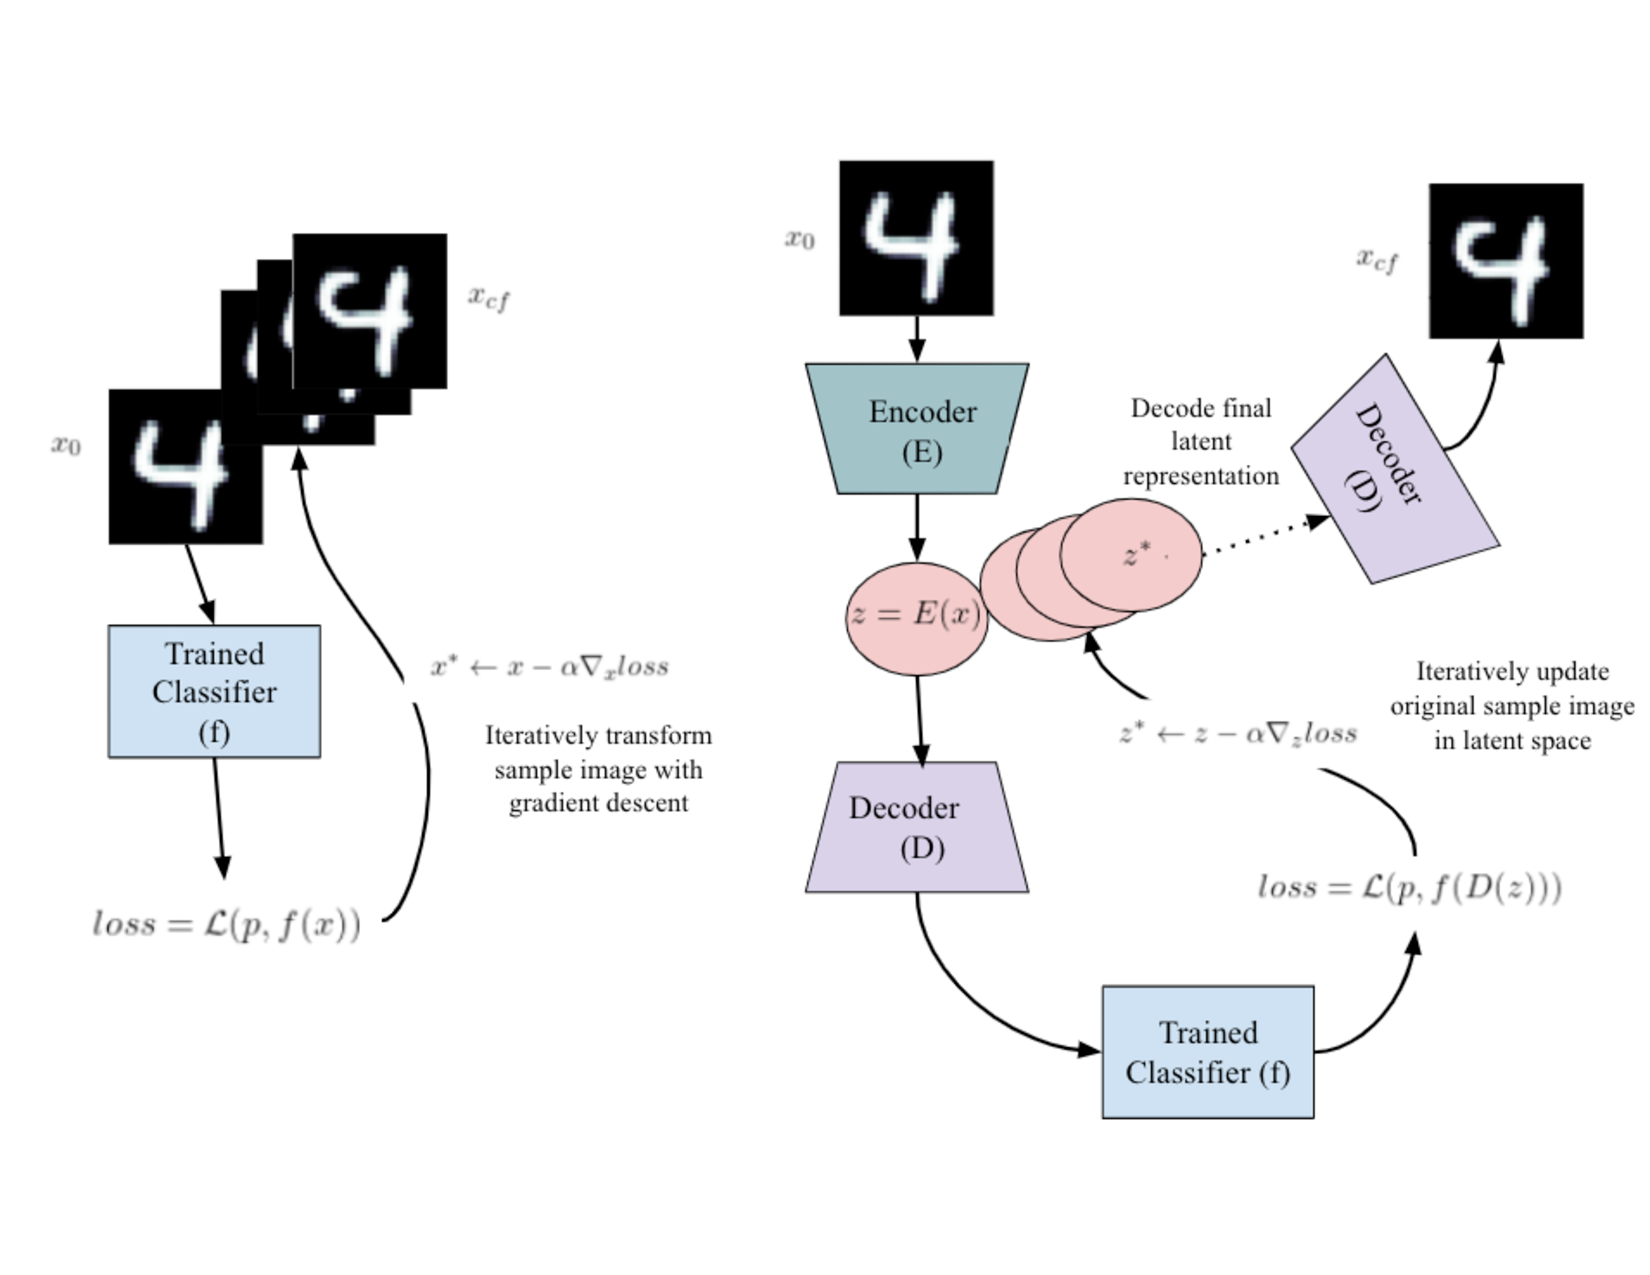
\includegraphics[width=0.99\linewidth,trim=30 75 0 85]{figures/mnist/Architecture}
    \caption{Comparing approaches for counterfactual generation between gradient descent in feature space (left) and Latent-CF gradient descent in the autoencoder latent space (right)}
    \label{fig:arch}
\end{figure}

\subsection{Baseline Methods}
Our first baseline method, \textit{Feature GD}, uses gradient descent to directly perturb the feature space minimizing the $\ell_{2}$ distance to the decision boundary. Two other methods introduce some small changes to make iterative improvements over Feature GD. First, we add feature clipping after every gradient step in \textit{Feature GD + clip} to ensure pixel values stay within the correct domain. 

% While this was a good initial method, we noticed many ways in which we could improve our counterfactual. To keep the counterfactual more in sample, we add clipping (Feature GD + clip) to prevent the pixel values from going below $0$ or above $1$, since these are the only values the pixels should be able to take. 
% % This can be accomplished by implementing clipping, limiting the range of values that the pixels could take on. 
% At the end of each gradient descent step, any pixels that are out of range will be clipped back to $0$ at minimum and $1$ at maximum.

We implement \textit{Feature GD + MAD loss}, which encourages in-sample counterfactuals and sparse changes with Median Absolute Deviation (MAD) scaling loss, as developed by Wachter et al~\cite{wachter2017counterfactual}. Instead of the $\ell_2$ loss, this method uses the $\ell_1$ norm weighted by the inverse median absolute deviation, such that $MAD_k$ of a feature $k$ over the set of points $P$ is as shown in equation~\ref{eq:mad}.
\begin{equation}
    {MAD}_k = median_{j\in{P}}(|X_{j,k} - median_{l\in{P}}(X_{l,k})|)
    \label{eq:mad}
\end{equation}

This results in a distance metric $d$ for between a synthetic data point $x'$ and original data point $x$ as described by equation 2.
\begin{equation}
    d(x, x') = \sum_{k\in{F}}\frac{|x_k-x'_k|}{MAD_k}
\end{equation}

This distance metric encourages changing only the pixels that vary in the training set, and punishes changing the border pixels that are rarely nonzero.The architecture for these three methods is illustrated on the left of Figure~\ref{fig:arch}.

We compare a final feature gradient descent method from \cite{looveren2019interpretable} which we label \textit{Prototype-CF}. The authors include five different loss terms in their objective to achieve desirable properties of their counterfactuals. $$ L = cL_{pred} + \beta L_1 + L_2 + L_{AE} + L_{proto}$$ $L_{pred}$ is designed to encourage counterfactuals of a different class. $L_1$ and $L_2$ are combined to form an elastic-net regularizer on the feature perturbations for sparse changes. They include $L_{AE}$ as used by Dhurandhar et al.~\cite{dhurandhar2018tip} to ensure in-sample reconstructions of counterfactuals. Finally, they guide the search for counterfactuals by introducing \textit{prototypes}, which are the average euclidean representation of a class in the latent space defined by the $K$ closest encoded samples to $E(x_0)$. Specifically, for a class $i$ the prototype is defined as $$proto_i = \frac{1}{K}\sum_{k=1}^K E(x_k^i)$$ where $\left\Vert E(x_k^i) - E(x_0)\right\Vert_2 \leq \left\Vert E(x_{k+1}^i) - E(x_0)\right\Vert_2$. $L_{proto}$, defined as the distance to the closest prototype, effectively tries to speed up the search for counterfactuals by pushing $x_0 +\delta$ to the closest prototype. 

% Having examined these methods, we explored doing gradient descent in latent space. Using an architecture as described in the right hand side of Figure 1. We trained an autoencoder on training data from MNIST, then when doing gradient descent calculated loss based on the images encoded by the encoder of the autoencoder, instead of the original features.

% Through all of these methods, we examined sparsity, how in sample it was, and how computationally efficient they were, as will be detailed in the results and discussion section.


\subsection{Evaluation Metrics}
In order to evaluate the quality of the counterfactual,  we use three evaluation metrics:


\textbf{1) In-distribution} \\
\noindent The counterfactual should not change the image such that proposed features will have a low probability of occurring. We used per-pixel intensity kernel density estimation (KDE) to measure the extent to which our counterfactuals are in-sample. Specifically, we estimate the density over intensity values for each pixel across the target class population. We compute the probability for each pixel intensity given the pixel specific KDE and take the average over all pixels. An example of this can be seen in Figure~\ref{fig:kde} comparing probabilities of pixels in counterfactuals as well as probabilities of the original pixels. 

\begin{figure}[hbt!]
  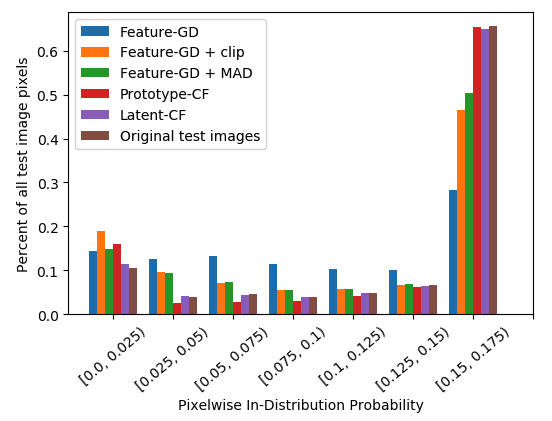
\includegraphics[width=0.48\textwidth]{figures/mnist/hist.png}
  \caption{Histogram of Kernel Density Estimate probabilities per pixel computed on original images and counterfactuals. In this case the counterfactual images generated by baseline methods have more low probability pixels than the original images, signifying out of distribution changes.}
  \label{fig:kde}
\end{figure}



\textbf{2) Sparsity} \\
\noindent The counterfactual should be sparse in the number of changes it makes in the features. We compute the percent of features that are changed in the generation of the counterfactual.

\textbf{3) Computational Efficiency} \\
\noindent Generating the counterfactual must be computationally efficient. We measure the time it takes to generate a counterfactual.


\subsection{Experiments}
%In order to demonstrate our methods of counterfactual generation as a baseline, we use the MNIST image dataset. 

In order to generate a baseline comparison of the counterfactual methods, we analyze the MNIST digit classification dataset. We performed a series of experiments. We first compare each method outlined above as well as the method proposed in \cite{looveren2019interpretable} on the four criteria proposed. As mentioned in Section~\ref{sec:models}, we use a convolutional neural network for the binary classification task of distinguishing fours and nines. Given this classifier, we generate counterfactuals for fours given nines and vice versa. We also conduct a visual comparison of the counterfactual images generated by each model type, and use these along with our evaluation metrics to draw conclusions about the quality of each method.

% Explain the architecture of the classifier and temperature calibration

% Secondly, we explore how robustness of fit would affect the generation of counterfactuals. In order to test this, we trained a variety of models with differing levels of fit, from overfit to underfit. To do this, we limited the amount of training data and increased model complexity to overfit, and then added weight decay to tune the models back to wellfit, and then further to underfit. 

% \textbf{(This sounds like you are overfitting first, then tuning that same model, is that correct? Or are these trained from scratch each time?)}

% Thirdly, we look at the impact of the classifier's calibration on the generation of counterfactuals by comparing poorly calibrated models with those calibrated using temperature scaling, since convolutional models are known to be susceptible to becoming uncalibrated. 

\section{Results and Discussion}
\begin{table}[ht]
\centering
\begin{tabular}{l|c|c|c|c}
\textbf{Method}         & \textbf{In-Distribution}  & \textbf{Sparsity (\%) } & \textbf{Time (s)} \\ \hline
Feature GD                  & 0.098         &  77.5     &      \textbf{0.346}        \\ \hline
Feature GD + clip           & 0.111        &  48.7      &      0.401         \\ \hline
Feature GD + MAD loss       & 0.117        &  38.4      &      0.364        \\ \hline
Prototype-CF                & 0.133  &  \textbf{16.8} &      15.400         \\ \hline
Latent-CF           & \textbf{0.135} &      24.2&      1.134  
\end{tabular}
\caption{Mean and standard deviation for quality metrics given a target counterfactual class probability of 0.5: in-distribution, sparsity, and time for all methods in this study. }
\label{tab:comparison}
\end{table}

In Table~\ref{tab:comparison}, we present a comparison of each method across all of the proposed metrics. Each of these metrics were calculated using a fixed probability, $p = 0.5$,   as the decision boundary. We will investigate each metric in further detail later on, but this serves to point out some immediate trends. First, we can notice that by far Prototype-CF method takes much longer than the Feature GD methods. Secondly, we notice that Latent-CF and the Prototype-CF method change a much smaller percentage of the pixels, making their generated counterfactuals sparser. Finally, Prototype-CF and Latent-CF result in less out-of-distribution changes to the image resulting in in-distribution scores close the original images themselves (0.137).


\begin{figure}[hbt!]
    \centering
    \centering
    \begin{subfigure}{0.5\textwidth}
       \centering
        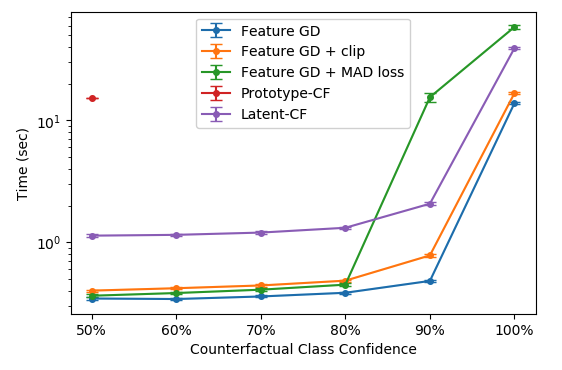
\includegraphics[width=0.9\linewidth]{figures/mnist/time.png}
        \caption{Counterfactual run time for each method}
        \label{fig:times}
    \end{subfigure}%
    \begin{subfigure}{0.5\textwidth}
      \centering
        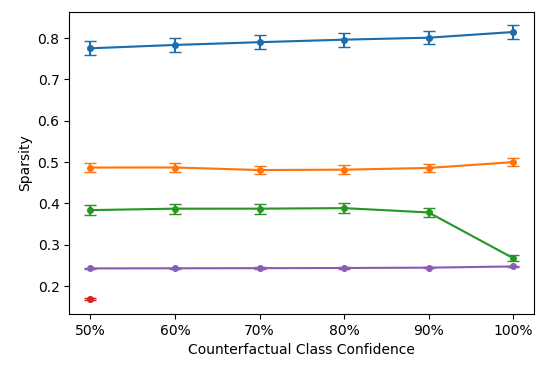
\includegraphics[width=0.9\linewidth]{figures/mnist/sparsity.png}
        \caption{Fraction of pixels changed by each method}
        \label{fig:pixels}
    \end{subfigure}
    
    \begin{subfigure}{0.5\textwidth}
        \centering
        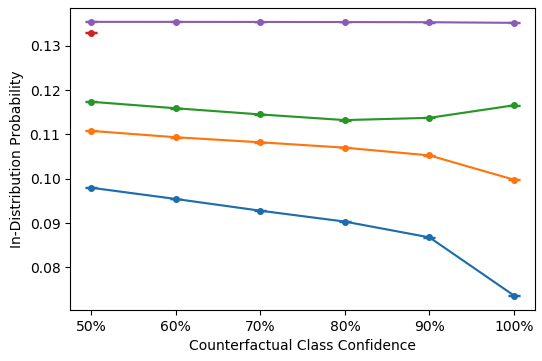
\includegraphics[width=0.9\linewidth]{figures/mnist/kde.png}
        \caption{In-distribution probability over all test image pixels}
        \label{fig:kde_confidences}
    \end{subfigure}
    \caption{Average and 95\% CI of time, sparsity, and in-distribution probability across all test images calculated for various counterfactual confidence levels.} %Note that Latent-CF is not effected by desired confidence in sparsity and pixel likelihood while other methods are.}
    \label{fig:confidences}
\end{figure}

In Figure~\ref{fig:confidences} we show these performance metrics when pushing beyond the decision boundary of 0.5 to higher levels confidence. We only include results for Prototype-CF at 0.5 since their formulation uses a penalty to encourage bounding the confidence from below. Figure ~\ref{fig:kde_confidences} shows how the probability of being in sample changes for different confidence values. Models that perform gradient descent in feature space tend to drift more out of sample as the classifier seeks to obtain higher confidence in the counterfactual image, while the Latent-CF method stays relatively stable. We notice that for most Feature GD counterfactuals, the changes are somewhat adversarial in that they make a significant number of perturbations around the border of the image. These changes get larger in magnitude as we target higher confidences, thus decreasing average pixel in-distribution probability. 

To get a quantitative evaluation of how each model and method performed in terms of sparsity, we calculated the fraction of the 784 pixels that were changed to get from the original image to the counterfactual image. Figure~\ref{fig:pixels} demonstrates how the proportion of pixels changed varies with increasing confidence.

% be careful with the trailing percent signs - they control newlines
\begin{figure}[hbt!]
    \centering
    \begin{subfigure}{0.6\textwidth}
        \centering
        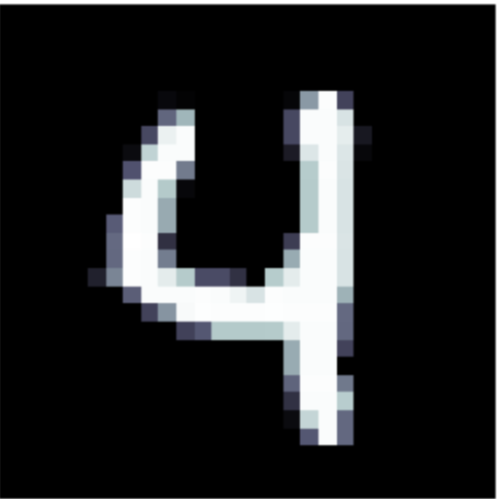
\includegraphics[width=0.4\linewidth]{figures/mnist/original.png}
        \caption{Original Image}
        \label{fig:original}
    \end{subfigure}
    \begin{subfigure}{0.5\textwidth}
        \centering
        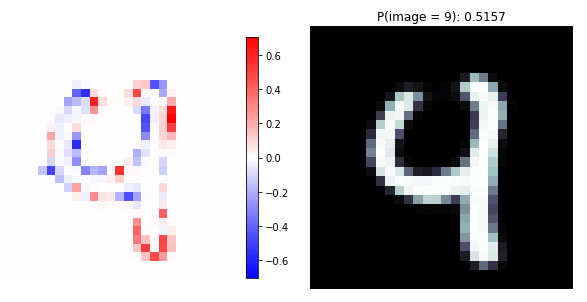
\includegraphics[width=0.99\linewidth]{figures/mnist/latent.png}
        \caption{Latent-CF}
        \label{fig:latent}
    \end{subfigure}
    \begin{subfigure}{0.5\textwidth}
        \centering
        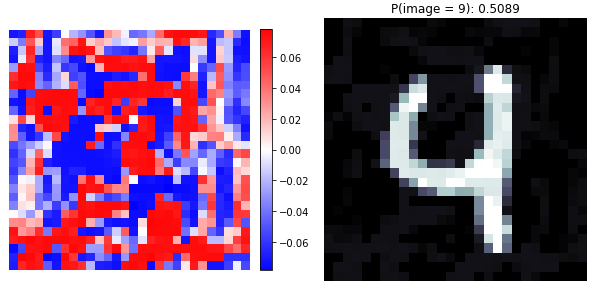
\includegraphics[width=0.99\linewidth]{figures/mnist/simple.png}
        \caption{feature gradient descent}
        \label{fig:simple}
    \end{subfigure}%
    \begin{subfigure}{0.5\textwidth}
        \centering
        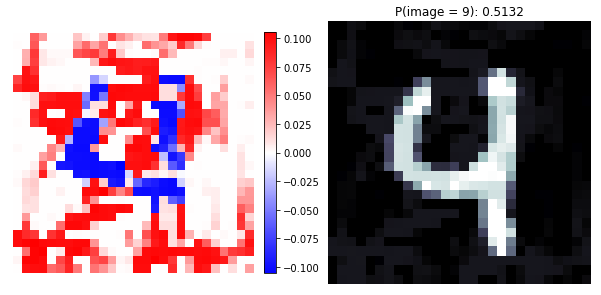
\includegraphics[width=0.99\linewidth]{figures/mnist/clip.png}
        \caption{feature gradient descent with clipping}
        \label{fig:clipping}
    \end{subfigure}
    \begin{subfigure}{0.5\textwidth}
        \centering
        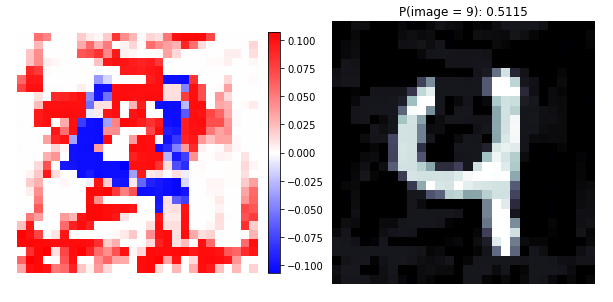
\includegraphics[width=0.99\linewidth]{figures/mnist/mad.png}
        \caption{MAD loss}
        \label{fig:wachter}
    \end{subfigure}%
    \begin{subfigure}{0.5\textwidth}
        \centering
        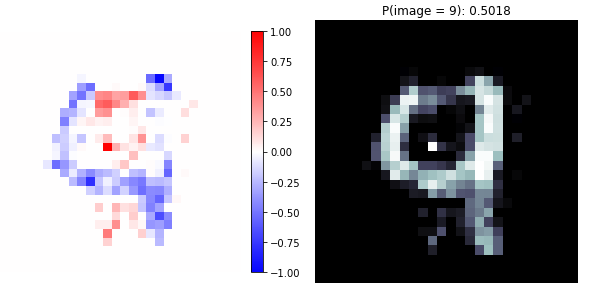
\includegraphics[width=0.99\linewidth]{figures/mnist/proto.png}
        \caption{Prototype-CF}
        \label{fig:proto}
    \end{subfigure}
    \caption{Visual inspection of counterfactual generation by each of the four methods proposed here. The heat map corresponds to the changes in intensities of each pixel. Note smaller scales for feature gradient descent methods. }
    \label{fig:images}
\end{figure}


Finally, efficiency is important when generating counterfactuals for production systems. Table~\ref{tab:comparison} shows the time in seconds that it took for each model type to generate a counterfactual with a given method. Unsurprisingly, the feature gradient descent methods tend to run the fastest and methods that add additional transformations, architectures, or losses increases the computation necessary and slows down counterfactual generation. We also see these effects across levels of counterfactual confidence in Figure~\ref{fig:times}. Latent-CF strikes a balance between all the elements of a quality counterfactual generation method. Latent-CF demonstrates the advantages of Prototype-CF while also resulting in an order of magnitude speed up.

We also provide a visual examination of counterfactuals in Figure~\ref{fig:images}. We start with an image classified as a 4 (Figure~\ref{fig:original}) and generate counterfactual images with each method. We include the counterfactual image and heat map which illustrates the addition or subtraction of luminosity for a pixel in the counterfactual image compared to the original. These are presented for each of the four described methods in Figures \ref{fig:latent} to \ref{fig:proto}. From the heat maps, we can observe that the initial attempt using feature gradient descent is noisy and does not seem to be confined to any features of the 4. Once we add clipping, we do observe a less noisy heat map, with aspects of the 4 becoming visible, but there are still many noisy changes in surrounding pixels. Using MAD loss results in similar changes as clipping. Finally, we can observe that Latent-CF and Prototype-CF actually begin to modify the shape of the four, adding curvature and closing the top of the of the four as could be expected in a nine. We can see a significant change in the heat map as Latent-CF directly manipulates the shape of the four as changes are concentrated on the border of the four while Prototype-CF makes some extraneous changes inside and outside the main shape. 


\section{Conclusions}
We demonstrate the benefits of performing perturbations in a representative latent space compared to various methods in feature space for counterfactual generation. We show that these methods benefit from sparsity and in-sample perturbations that simple feature based methods lack. Latent based generation also exhibits significant speed up compared to more complex feature based methods designed to remedy simple methods' difficulty generating sparse and in-sample counterfactuals.



\section{ Acknowledgments}

\bibliography{latent_cf}
\end{document}
